\documentclass{beamer}
%
\mode<presentation>
{
  \usetheme{default}
  \usecolortheme{default}
  \usefonttheme{default}
  \setbeamertemplate{navigation symbols}{}
  \setbeamertemplate{caption}[numbered]
}

\usepackage[english]{babel}
\usepackage[utf8]{inputenc}
\usepackage[T1]{fontenc}
\usepackage{lmodern}
\usepackage{amsmath}
\usepackage{amssymb}
\usepackage{graphicx}

\title[Sample Presentation]{Presentation of References 1}
\author{Shanik Hubert}
\institute{}
\date{}

\begin{document}

\begin{frame}{}
    \titlepage
\end{frame}

\begin{frame}{Contents}
  \tableofcontents
\end{frame}

\begin{frame}{Paper 1}
M. Kim, J. Park and J. Lee, ``MU-MIMO Precoding Design in the Presence of Delay-Constrained Users,'' ICC 2021 - IEEE International Conference on Communications, Montreal, QC, Canada, 2021,
\end{frame}

\section{Precoding Design for Multi-user MIMO Systems with Delay-Constrained and Delay-Tolerant Users}

\begin{frame}{Introduction: DCTU-MIMO Precoding}

\begin{block}{Abstract}
This paper studies precoding design for multi-user MIMO systems serving both delay-constrained and delay-tolerant users. The objective is to maximize the ergodic sum spectral efficiency while satisfying latency and reliability requirements under finite blocklength transmission. A generalized power iteration (GPI) based precoding method is used to efficiently handle the resulting non-convex optimization problem. Numerical results show that the proposed Delay-GPI and Infinite-GPI schemes outperform conventional precoding methods such as RZF and MRT, especially under different user weights and delay constraints.
\end{block}

\end{frame}

\begin{frame}{System Overview}

\begin{itemize}
    \item A base station with $N$ antennas serves two types of users:
    \begin{itemize}
        \item \textbf{Delay-tolerant users:} require high spectral efficiency.
        \item \textbf{Delay-constrained users:} require strict latency guarantees.
    \end{itemize}

    \item A base station with $N$ antennas serves:
    \[
        K_t \text{ delay-tolerant users},
        \qquad
        K_s \text{ delay-constrained users}
    \]

    \item Total user set:
    \[
        \mathcal{K} = \mathcal{K}_t \cup \mathcal{K}_s
    \]

    \item The transmitted signal is precoded as:
    \[
        \mathbf{x} = \sum_{k=1}^{K_t+K_s} \mathbf{u}_k s_k
    \]
    where $\mathbf{u}_k$ is the precoding vector for user $k$.

    \item The received signal at user $k$ is:
    \[
        y_k = \mathbf{h}_k^H \mathbf{u}_k s_k
        + \sum_{i\neq k}\mathbf{h}_k^H \mathbf{u}_i s_i
        + z_k
    \]

    \item Objective: maximize delay-tolerant users' sum spectral efficiency while satisfying delay-constrained users' latency requirement:
    \[
        \max_{\mathbf{u}} \sum_{k=1}^{K_t} R_k(\mathbf{u})
        \quad
        \text{s.t.}
        \quad
        \tilde{R}_k(\mathbf{u},\tilde{\gamma}_k)
        \geq
        \frac{D_s}{\delta_k},
        \quad k\in \mathcal{K}_s
    \]
\end{itemize}
\end{frame}

\begin{frame}{}

\begin{itemize}
    \item The paper solves this non-convex problem using a generalized power iteration method called \textbf{Delay-GPI}.
\end{itemize}

\end{frame}

\begin{frame}{Spectral Efficiency Modeling}

\begin{itemize}
    \item The SINR of user $k$ is:
    \[
        \gamma_k =
        \frac{
        |\mathbf{h}_k^H \mathbf{u}_k|^2
        }{
        \sum_{i\neq k}|\mathbf{h}_k^H \mathbf{u}_i|^2
        +
        \frac{\sigma_k^2}{P}
        }
    \]

    \item For delay-tolerant users, Shannon capacity is used:
    \[
        R_k(\gamma_k)=\log_2(1+\gamma_k),
        \qquad k\in \mathcal{K}_t
    \]

    \item For delay-constrained users, finite blocklength rate is used:
    \[
        R_k(\gamma_k)
        =
        \log_2(1+\gamma_k)
        -
        \sqrt{\frac{V(\gamma_k)}{m}}Q^{-1}(\epsilon_k),
        \qquad k\in \mathcal{K}_s
    \]

    \item Here, $m$ is blocklength and $\epsilon_k$ is target error probability.

    \item The second term is the finite blocklength penalty, which reduces the achievable rate for low-latency users.

\end{itemize}

\end{frame}

\begin{frame}{Rayleigh Quotient Reformulation}
\small

\begin{itemize}
    \item A Rayleigh quotient is a quadratic matrix ratio of the form:
    \[
        \frac{\mathbf{x}^H\mathbf{A}\mathbf{x}}
        {\mathbf{x}^H\mathbf{B}\mathbf{x}}
    \]

    \item Here:
    \[
        \mathbf{x} = \text{optimization vector},
        \qquad
        \mathbf{A},\mathbf{B} = \text{matrices}
    \]

    \item In this paper, the optimization vector is the stacked precoder:
    \[
        \mathbf{u}
        =
        [\mathbf{u}_1^H,\mathbf{u}_2^H,\ldots,
        \mathbf{u}_{K_t+K_s}^H]^H
    \]

    \item Therefore, the Rayleigh quotient becomes:
    \[
        \frac{\mathbf{u}^H\mathbf{A}_k\mathbf{u}}
        {\mathbf{u}^H\mathbf{B}_k\mathbf{u}}
    \]

    \item This quotient represents:
    \[
        \frac{\text{signal + interference + noise}}
        {\text{interference + noise}}
        =
        1+\gamma_k
    \]

    \item This allows us to apply the GPI algorithm (as it makes it easier to reformulate into an eigenvalue problem formulation).

\end{itemize}

\end{frame}

\begin{frame}{}

\begin{itemize}
    \item Start with the SINR of user $k$:
    \[
        \gamma_k =
        \frac{
        |\mathbf{h}_k^H\mathbf{u}_k|^2
        }{
        \sum_{i\neq k}|\mathbf{h}_k^H\mathbf{u}_i|^2
        +
        \frac{\sigma_k^2}{P}
        }
    \]

    \item Hence:
    \[
        1+\gamma_k
        =
        \frac{
        \sum_{i=1}^{K_t+K_s}|\mathbf{h}_k^H\mathbf{u}_i|^2
        +
        \frac{\sigma_k^2}{P}
        }{
        \sum_{i\neq k}|\mathbf{h}_k^H\mathbf{u}_i|^2
        +
        \frac{\sigma_k^2}{P}
        }
    \]

    \item Define the stacked precoding vector:
    \[
        \mathbf{u}
        =
        [\mathbf{u}_1^H,\mathbf{u}_2^H,\ldots,
        \mathbf{u}_{K_t+K_s}^H]^H
    \]

\end{itemize}

\end{frame}

\begin{frame}{\(\mathbf{A}_k\) and \(\mathbf{B}_k\)}
\small

\begin{itemize}
    \item Let:
    \[
        K = K_t + K_s,
        \qquad
        \mathbf{H}_k = \mathbf{h}_k\mathbf{h}_k^H
    \]

    \item The matrix $\mathbf{A}_k$ contains all received signal power terms:
    \[
        \mathbf{A}_k
        =
        \mathrm{diag}
        (\mathbf{H}_k,\mathbf{H}_k,\ldots,\mathbf{H}_k)
        +
        \frac{\sigma_k^2}{P}\mathbf{I}_{NK}
    \]

    \item Therefore:
    \[
        \mathbf{u}^H\mathbf{A}_k\mathbf{u}
        =
        \sum_{i=1}^{K}
        |\mathbf{h}_k^H\mathbf{u}_i|^2
        +
        \frac{\sigma_k^2}{P}
    \]
    \[
        =
        \text{desired signal + interference + noise}
    \]

    \item The matrix $\mathbf{B}_k$ removes the desired signal block of user $k$:
    \[
        \mathbf{B}_k
        =
        \mathbf{A}_k
        -
        \mathrm{diag}
        (0,\ldots,\mathbf{H}_k,\ldots,0)
    \]

    \item Hence:
    \[
        \mathbf{u}^H\mathbf{B}_k\mathbf{u}
        =
        \sum_{i\neq k}
        |\mathbf{h}_k^H\mathbf{u}_i|^2
        +
        \frac{\sigma_k^2}{P}
    \]
    \[
        =
        \text{interference + noise}
    \]
\end{itemize}
\end{frame}

\begin{frame}{}
\begin{itemize}
    \item Thus:
    \[
        \frac{\mathbf{u}^H\mathbf{A}_k\mathbf{u}}
        {\mathbf{u}^H\mathbf{B}_k\mathbf{u}}
        =
        \frac{\text{signal + interference + noise}}
        {\text{interference + noise}}
        =
        1+\gamma_k
    \]
\end{itemize}
\end{frame}

\begin{frame}{}

\begin{itemize}
    \item For delay-tolerant users, Shannon capacity is used directly since they are assumed to have long blocklength:
    \[
        R_k(\mathbf{u})
        =
        \log_2
        \left(
        \frac{\mathbf{u}^H\mathbf{A}_k\mathbf{u}}
        {\mathbf{u}^H\mathbf{B}_k\mathbf{u}}
        \right),
        \qquad k\in\mathcal{K}_t
    \]

    \item For delay-constrained users, finite blocklength coding is used:
    \[
        R_k(\gamma_k)
        =
        \log_2(1+\gamma_k)
        -
        \sqrt{\frac{V(\gamma_k)}{m}}Q^{-1}(\epsilon_k)
    \]

    \item Since this is difficult to optimize, the paper uses the lower bound(derivation is in the paper):
    \[
        \tilde{R}_k(\mathbf{u},\tilde{\gamma}_k)
        =
        \log_2
        \left[
        \left(
        \frac{\mathbf{u}^H\mathbf{A}_k\mathbf{u}}
        {\mathbf{u}^H\mathbf{B}_k\mathbf{u}}
        \right)^{1-f_k(\tilde{\gamma}_k)}
        \right]
        -
        g_k(\tilde{\gamma}_k)
    \]

    \item Therefore, the Rayleigh quotient is used for both user types.
\end{itemize}

\end{frame}

\begin{frame}{First-Order Optimality Condition (1): Lagrangian Setup}
\small

\begin{itemize}
    \item The optimization problem is:
    \[
        \max_{\mathbf{u}}
        \sum_{k=1}^{K_t} R_k(\mathbf{u})
    \]
    \[
        \text{s.t.}
        \quad
        \tilde{R}_k(\mathbf{u},\tilde{\gamma}_k)
        \geq
        \frac{D_s}{\delta_k},
        \qquad k\in\mathcal{K}_s .
    \]
    \item Only sum rate of delay tolerant users are optimized, rate of delay constrained users just need to be enough to satisfy latency constraints.  
    \item $D_s$ is the data size of downlink signal, $\delta_k$ is latency of user $k$.

    \item Convert maximization into minimization:
    \[
        \min_{\mathbf{u}}
        -
        \sum_{k=1}^{K_t} R_k(\mathbf{u})
    \]

    \item Introduce Lagrange multiplier $\lambda_k$ for each delay-constrained user:
    \[
        \lambda_k \geq 0,
        \qquad k\in\mathcal{K}_s .
    \]

\end{itemize}
\end{frame}

\begin{frame}
\begin{itemize}
    \item Lagrangian:
    \[
        \mathcal{L}(\mathbf{u},\lambda)
        =
        -
        \sum_{k=1}^{K_t} R_k(\mathbf{u})
        -
        \sum_{k=K_t+1}^{K_t+K_s}
        \lambda_k
        \left[
        \tilde{R}_k(\mathbf{u},\tilde{\gamma}_k)
        -
        \frac{D_s}{\delta_k}
        \right].
    \]

    \item $\lambda_k$ controls how strongly the latency constraint affects the precoder.
\end{itemize}

\end{frame}

\begin{frame}{First-Order Optimality Condition (2): Substituting Rate Expressions}
\small

\begin{itemize}
    \item Delay-tolerant user rate:
    \[
        R_k(\mathbf{u})
        =
        \log_2
        \left(
        \frac{\mathbf{u}^H\mathbf{A}_k\mathbf{u}}
        {\mathbf{u}^H\mathbf{B}_k\mathbf{u}}
        \right)
    \]

    \item Delay-constrained lower-bound rate:
    \[
        \tilde{R}_k(\mathbf{u},\tilde{\gamma}_k)
        =
        \log_2
        \left[
        \left(
        \frac{\mathbf{u}^H\mathbf{A}_k\mathbf{u}}
        {\mathbf{u}^H\mathbf{B}_k\mathbf{u}}
        \right)^{1-f_k}
        \right]
        -
        g_k .
    \]

    \item Substituting into the Lagrangian:
    \[
        \mathcal{L}
        =
        -
        \sum_{k=1}^{K_t}
        \log_2
        \left(
        \frac{\mathbf{u}^H\mathbf{A}_k\mathbf{u}}
        {\mathbf{u}^H\mathbf{B}_k\mathbf{u}}
        \right)
    \]
    \[
        -
        \sum_{k=K_t+1}^{K_t+K_s}
        \lambda_k
        \left[
        \log_2
        \left(
        \frac{\mathbf{u}^H\mathbf{A}_k\mathbf{u}}
        {\mathbf{u}^H\mathbf{B}_k\mathbf{u}}
        \right)^{1-f_k}
        -
        g_k
        -
        \frac{D_s}{\delta_k}
        \right].
    \]

    \item The terms $g_k$(rewritten as a constant while defining the lower bound) and $\frac{D_s}{\delta_k}$ do not depend on $\mathbf{u}$.
\end{itemize}

\end{frame}

\begin{frame}{First-Order Optimality Condition (3): Grouping and Differentiation}
\small

\begin{itemize}
    \item Using $\sum \log(x_k)=\log\left(\prod x_k\right)$, group all $\mathbf{u}$-dependent terms as:
    \[
        \mathcal{L}(\mathbf{u},\lambda)
        =
        -\log_2 \phi(\mathbf{u},\lambda)
        +
        \text{constant terms}
    \]

    \item where:
    \[
        \phi(\mathbf{u},\lambda)
        =
        \frac{
        \prod_{k=1}^{K_t}
        \mathbf{u}^H\mathbf{A}_k\mathbf{u}
        \prod_{k=K_t+1}^{K_t+K_s}
        (\mathbf{u}^H\mathbf{A}_k\mathbf{u})^{\lambda_k(1-f_k)}
        }
        {
        \prod_{k=1}^{K_t}
        \mathbf{u}^H\mathbf{B}_k\mathbf{u}
        \prod_{k=K_t+1}^{K_t+K_s}
        (\mathbf{u}^H\mathbf{B}_k\mathbf{u})^{\lambda_k(1-f_k)}
        } .
    \]

    \item First-order condition:
    \[
        \frac{\partial \mathcal{L}}{\partial \mathbf{u}^H}=0
    \]

    \item Since:
    \[
        \frac{\partial \mathcal{L}}{\partial \mathbf{u}^H}
        =
        -
        \frac{1}{\phi(\mathbf{u},\lambda)\ln 2}
        \frac{\partial \phi(\mathbf{u},\lambda)}
        {\partial \mathbf{u}^H},
    \]
    we get:
    \[
        \frac{\partial \phi(\mathbf{u},\lambda)}
        {\partial \mathbf{u}^H}=0 .
    \]

\end{itemize}
\end{frame}

\begin{frame}{}
\begin{itemize}
    \item Define:
    \[
        \phi = \frac{N}{D},
        \qquad
        \frac{\partial N}{\partial \mathbf{u}^H}
        =
        \bar{\mathbf{A}}(\mathbf{u},\lambda)\mathbf{u},
        \qquad
        \frac{\partial D}{\partial \mathbf{u}^H}
        =
        \bar{\mathbf{B}}(\mathbf{u},\lambda)\mathbf{u}
    \]
    \item This leads to:
    \[
        \bar{\mathbf{A}}(\mathbf{u},\lambda)\mathbf{u}
        =
        \phi(\mathbf{u},\lambda)
        \bar{\mathbf{B}}(\mathbf{u},\lambda)\mathbf{u}.
    \]

    \item This is a generalized eigenvalue-type condition solved using Delay-GPI.
\end{itemize}

\end{frame}

\begin{frame}{Delay-GPI Precoding Algorithm}

\begin{itemize}
    \item From the first-order condition:
    \[
        \bar{\mathbf{A}}(\mathbf{u},\lambda)\mathbf{u}
        =
        \phi(\mathbf{u},\lambda)
        \bar{\mathbf{B}}(\mathbf{u},\lambda)\mathbf{u}
    \]

    \item This resembles a generalized eigenvalue problem:
    \[
        \mathbf{A}\mathbf{u}=\mu \mathbf{B}\mathbf{u}
    \]

    \item However, $\bar{\mathbf{A}}$ and $\bar{\mathbf{B}}$ depend on $\mathbf{u}$ itself.

    \item Therefore, the paper uses an iterative generalized power iteration method.

    \item Precoder update:
    \[
        \mathbf{u}^{(j)}
        =
        \left[
        \bar{\mathbf{B}}(\mathbf{u}^{(j-1)},\lambda^{(n)})
        \right]^{-1}
        \bar{\mathbf{A}}(\mathbf{u}^{(j-1)},\lambda^{(n)})
        \mathbf{u}^{(j-1)}
    \]

    \item Normalize:
    \[
        \mathbf{u}^{(j)}
        =
        \frac{\mathbf{u}^{(j)}}{\|\mathbf{u}^{(j)}\|}
    \]

\end{itemize}

\end{frame}

\begin{frame}{Delay-GPI Algorithm (2): Why Direct Eigenvalue Solution Fails}
\small

\begin{itemize}
    \item If $\bar{\mathbf{A}}$ and $\bar{\mathbf{B}}$ were fixed, we could write:
    \[
        \bar{\mathbf{B}}^{-1}\bar{\mathbf{A}}\mathbf{u}
        =
        \phi \mathbf{u}
    \]

    \item This is a normal eigenvalue problem:
    \[
        \mathbf{M}\mathbf{u}
        =
        \phi \mathbf{u},
        \qquad
        \mathbf{M}
        =
        \bar{\mathbf{B}}^{-1}\bar{\mathbf{A}}
    \]

    \item But in this paper:
    \[
        \bar{\mathbf{A}}=\bar{\mathbf{A}}(\mathbf{u},\lambda),
        \qquad
        \bar{\mathbf{B}}=\bar{\mathbf{B}}(\mathbf{u},\lambda)
    \]

    \item So the matrices themselves depend on the unknown precoder $\mathbf{u}$.

    \item Therefore, the problem cannot be solved by one direct eigenvalue decomposition.

    \item The paper solves it iteratively using generalized power iteration.
\end{itemize}

\end{frame}

\begin{frame}{Delay-GPI Algorithm (3): Precoder Update}
\small

\begin{itemize}
    \item At iteration $j$, use the previous precoder $\mathbf{u}^{(j-1)}$ to construct:
    \[
        \bar{\mathbf{A}}
        \left(
        \mathbf{u}^{(j-1)},\lambda^{(n)}
        \right),
        \qquad
        \bar{\mathbf{B}}
        \left(
        \mathbf{u}^{(j-1)},\lambda^{(n)}
        \right)
    \]

    \item Then update the precoder as:
    \[
        \mathbf{u}^{(j)}
        =
        \left[
        \bar{\mathbf{B}}
        \left(
        \mathbf{u}^{(j-1)},\lambda^{(n)}
        \right)
        \right]^{-1}
        \bar{\mathbf{A}}
        \left(
        \mathbf{u}^{(j-1)},\lambda^{(n)}
        \right)
        \mathbf{u}^{(j-1)}
    \]

    \item Normalize after each update:
    \[
        \mathbf{u}^{(j)}
        =
        \frac{\mathbf{u}^{(j)}}{\|\mathbf{u}^{(j)}\|}
    \]

    \item Normalization satisfies the total transmit power constraint (which is assumed to be 1).
\end{itemize}

\end{frame}

\begin{frame}{Delay-GPI: Feasibility and Convergence}
\small

\begin{itemize}
    \item The Delay-GPI algorithm may not always find a feasible precoder.

    \item Feasibility depends on system parameters such as:
    \[
        P,\quad \epsilon_k,\quad D_s,\quad \delta_k,\quad \mathbf{h}_k
    \]

    \item If a delay-constrained user has weak channel gain, the BS may need more transmit power to satisfy:
    \[
        \tilde{R}_k(\mathbf{u},\tilde{\gamma}_k)
        \geq
        \frac{D_s}{\delta_k}
    \]

    \item If the required latency is too strict or transmit power is too low, the constraint may be infeasible.

    \item In that case, the delay-constrained user is assumed to fail transmission
    and its contribution is not added to the ergodic sum spectral efficiency.

    \item The precoder update continues until the convergence criterion is satisfied:
    \[
        \left\|
        \mathbf{u}^{(j)}
        -
        \mathbf{u}^{(j-1)}
        \right\|
        <
        \xi
    \]

    \item Here, $\xi$ is a small tolerance value that controls when the iterative update stops.

    \item Final output:
    \[
        \mathbf{u}^{\star}=\mathbf{u}^{(j)}
    \]

\end{itemize}

\end{frame}

\begin{frame}{Results - 1}
\begin{figure}
    \centering
    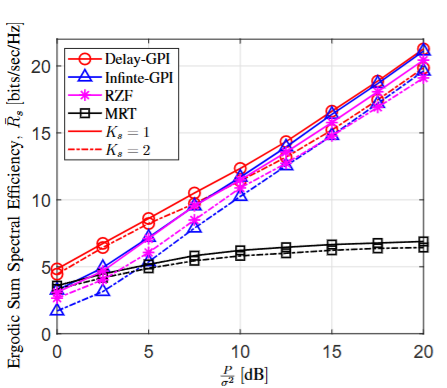
\includegraphics[width=0.75\linewidth]{image.png}
    \label{fig:placeholder1}
    \caption{Ergodic sum spectral efficiency $\bar{R}_s$ as a function of $P/2$ with $m = 100$ $N = 8$ and $K_t = 3$ for different values of $K_s$. In the case of $K_s = 1$, $\delta_4 = 250$. When $K_s = 2$, $\delta_4 = 250$ and $\delta_5 = 450$.}
\end{figure}

\end{frame}

\begin{frame}{Results - 2}
\begin{figure}
    \centering
    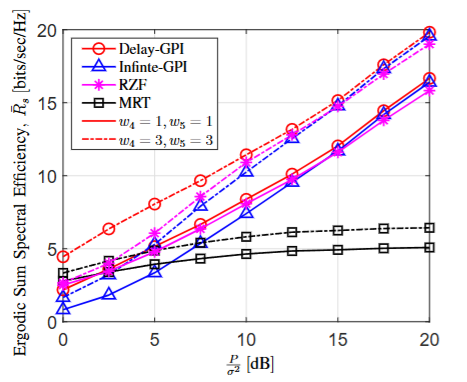
\includegraphics[width=0.75\linewidth]{image1.png}
    \caption{$\frac{P}{\sigma^2}$ with $m = 300$ $N = 8$, $K_t = 3$, $K_s = 2$,
$\delta_4 = 250$, $\delta_5 = 450$, $\tilde{\gamma}_4 = 2.38$, and
$\tilde{\gamma}_5 = 1.35$ for different values of $w_k$. $w_1, w_2, w_3 =1$}
    \label{fig:placeholder2}
\end{figure}

\end{frame}

\begin{frame}{Inference from Result 1: Effect of Number of Delay-Constrained Users}
\small

\begin{itemize}
    \item Result 1 compares the ergodic sum spectral efficiency for:
    \[
        K_s=1 \quad \text{and} \quad K_s=2
    \]
    with fixed (N is number of transmit antenna):
    \[
        N=8,\qquad K_t=3.
    \]

    \item Result:
    \[
        K_s \uparrow
        \quad \Rightarrow \quad
        \bar{R}_s \downarrow
    \]

    \item Reason: when more delay-constrained users are present, more transmit power must be reserved to satisfy:
    \[
        \tilde{R}_k(\mathbf{u},\tilde{\gamma}_k)
        \geq
        \frac{D_s}{\delta_k}.
    \]

    \item Therefore, less power remains for users with better channel gain.

    \item Delay-GPI still performs better because it explicitly considers finite blocklength latency constraints, while Infinite-GPI assumes:
    \[
        m=\infty
    \]
    during precoder design.
\end{itemize}

\end{frame}

\begin{frame}{Inference from Result 2: Effect of Delay-Constrained User Weights}
\small

\begin{itemize}
    \item Result 2 compares different weights for delay-constrained users:
    \[
        w_4=w_5=1
        \quad \text{and} \quad
        w_4=w_5=3.
    \]

    \item Larger weights increase the contribution of delay-constrained users in:
    \[
        R_s =
        \sum_{k=1}^{K_t} w_k R_k(\mathbf{u})
        +
        \sum_{k=K_t+1}^{K_t+K_s}
        p_{c,k} w_k \frac{D_s}{\delta_k}.
    \]

    \item Result:
    \[
        w_4,w_5 \uparrow
        \quad \Rightarrow \quad
        \text{Delay-GPI advantage becomes clearer.}
    \]

    \item When $w_4=w_5=1$, the gap between Delay-GPI and other methods decreases.

    \item At very low power, MRT/RZF may appear slightly better because Delay-GPI can fail to find a feasible precoder.

    \item However, Delay-GPI is more meaningful because it is designed to satisfy the latency constraints of delay-constrained users.
\end{itemize}

\end{frame}

\section{Adaptive Finite Blocklength for Ultra-Low Latency in Wireless Communications}

\begin{frame}{Paper 2}

W. Cheng, Y. Xiao, S. Zhang and J. Wang, ``Adaptive Finite Blocklength for Ultra-Low Latency in Wireless Communications,'' in IEEE Transactions on Wireless Communications, vol. 21, no. 6, pp. 4450-4463, June 2022,

\end{frame}

\begin{frame}{Introduction}
\small

\textbf{Paper:} Adaptive Finite Blocklength for Ultra-Low Latency in Wireless Communications

\vspace{0.2cm}

\textbf{Main problem:}
\begin{itemize}
    \item Future 6G systems require ultra-low end-to-end delay for autonomous vehicles, factory automation, remote control, and real-time machine--human interaction.
    \item Traditional LTE and 5G NR use fixed transmission time intervals (TTIs).
    \item The paper argues that fixed TTI is not always optimal for finite blocklength transmission.
\end{itemize}

\vspace{0.2cm}

\textbf{Main idea:}
\[
\text{Adapt the blocklength ie:  TTI to minimize delay.}
\]

\end{frame}

\begin{frame}{System Model}
\small

\begin{itemize}
    \item End-to-end delay:
\end{itemize}

\[
D_{\text{E2E}}
=
D_{\text{queue}}
+
D_{\text{trans}}
+
D_{\text{proc}}
+
D_{\text{prop}}
\]

\begin{itemize}
    \item Paper focuses on:
\end{itemize}

\[
D_{\text{queue}} + D_{\text{trans}}
\]

\begin{itemize}
    \item One frame = one TTI(transmission time interval).
    \item Blocklength:
\end{itemize}

\[
n = TB
\]

\[
T = \text{frame duration},
\qquad
B = \text{bandwidth}
\]

\begin{itemize}
    \item With fixed $B$:
\end{itemize}

\[
n \downarrow
\Rightarrow
T \downarrow
\Rightarrow
D_{\text{trans}} \downarrow
\]

\end{frame}

\begin{frame}{Finite Blocklength Rate and Queue Service}
\small

\begin{itemize}
    \item Finite blocklength achievable rate:
\end{itemize}

\[
R(n)
\approx
\log_2(1+P|h|^2)
-
\sqrt{\frac{V}{n}}Q^{-1}(\epsilon)\log_2 e
\]

\[
V = 1-(1+P|h|^2)^{-2}
\]

\begin{itemize}
    \item Information bits served in frame $i$:
\end{itemize}

\[
\text{served bits}_i = R(n_i)n_i
\]

\begin{itemize}
    \item If each packet has $a$ bits:
\end{itemize}

\[
\text{served packets}_i
=
\frac{R(n_i)n_i}{a}
\]

\begin{itemize}
    \item Shorter blocklength reduces rate:
\end{itemize}

\[
n_i \downarrow
\Rightarrow
R(n_i) \downarrow
\Rightarrow
R(n_i)n_i \downarrow
\Rightarrow
D_{\text{queue}} \uparrow
\]

\[
\boxed{
\text{Adaptive blocklength balances } D_{\text{trans}} \text{ and } D_{\text{queue}}.
}
\]

\end{frame}

\begin{frame}{Blocklength Tradeoff}
\begin{figure}
    \centering
    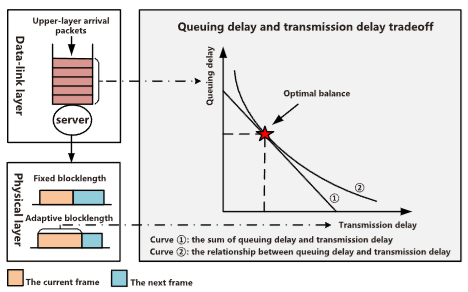
\includegraphics[width=0.5\linewidth]{image3.png}
    \label{fig:placeholder3}
\end{figure}
\small

\begin{itemize}
    \item Shorter blocklength means shorter frame duration: $n = TB$ where $T$ is transmission time interval(TTI) and $B$ is bandwidth(rate).

    \item Therefore, transmission delay decreases:$    n \downarrow \Rightarrow D_{\text{trans}} \downarrow
    $

    \item But in finite blocklength transmission, shorter blocklength reduces achievable rate:
    $
    n \downarrow \Rightarrow R(n) \downarrow
    $

    \item Lower rate means fewer packet bits per frame:
    $
    \text{served bits} = R(n)n
    $

    \item Therefore, packets wait longer in the buffer:
    \[
    R(n)n \downarrow \Rightarrow D_{\text{queue}} \uparrow
    \]
\end{itemize}

\[
\boxed{
\text{Adaptive blocklength balances transmission delay and queuing delay.}
}
\]

\end{frame}

\begin{frame}{Single-User Delay Model}
\small

\[
\mathbf{n} = (n_1,n_2,\ldots,n_L)
\]

\[
D_p
=
d_p
+
\sum_{j=1}^{I(p)-1} n_j
+
n_{I(p)}
=
d_p+\sum_{j=1}^{I(p)}n_j
\]

\begin{itemize}
    \item $N_p$: number of packets
    \item $L$: number of adaptive frames
    \item $I(p)$: frame that transmits packet $p$
    \item $d_p$: previous waiting time
\end{itemize}

\end{frame}

\begin{frame}{Single-User Delay Model}
\small

\begin{itemize}
    \item The user has $N_p$ short packets waiting in the buffer.
    \item These packets are transmitted over $L$ adaptive frames:
\end{itemize}

\[
\mathbf{n}=(n_1,n_2,\ldots,n_L)
\]

\begin{itemize}
    \item $n_i$ is the blocklength of frame $i$.
    \item If packet $p$ is transmitted in frame $I(p)$, it must wait for all previous frames.
\end{itemize}

\[
D_p
=
d_p
+
\sum_{j=1}^{I(p)-1} \frac{n_j}{B}
+
\frac{n_{I(p)}}{B}
=
d_p+\sum_{j=1}^{I(p)}\frac{n_j}{B}
\]

\begin{itemize}
    \item $d_p$: waiting time already accumulated from the previous period.
    \item $\sum_{j=1}^{I(p)-1}\frac{n_j}{B}$: queuing delay due to earlier frames.
    \item $\frac{n_{I(p)}}{B}$: transmission delay of the frame carrying packet $p$.
\end{itemize}

\end{frame}

\begin{frame}{Single-User Optimization Problem}
\small

\[
\begin{aligned}
\mathbf{F}_1:\quad
\min_{\mathbf{n}} \quad
& \frac{1}{N_p a}
\sum_{i=1}^{L}
R(n_i)n_i
\sum_{j=1}^{i} n_j \\[0.2cm]
\text{s.t.}\quad
& \sum_{i=1}^{L} R(n_i)n_i = N_p a,
&& \text{data-completion constraint} \\[0.1cm]
& \sum_{i=1}^{L} n_i \leq T_{\max},
&& \text{period-duration constraint} \\[0.1cm]
& n_i \geq 0,\quad i=1,2,\ldots,L,
&& \text{valid blocklength constraint}
\end{aligned}
\]

\begin{itemize}
    \item The objective represents the \textbf{average delay of all packets} served across $L$ frames.

    \item In frame $i$, the number of transmitted information bits is:
    \[
    R(n_i)n_i
    \]
\end{itemize}

\end{frame}

\begin{frame}{}
\begin{itemize}
    \item Since each packet has $a$ bits, the number of packets served in frame $i$ is:
    $
    \frac{R(n_i)n_i}{a}
    $

    \item Packets served in frame $i$ wait until frame $i$ finishes, so their delay is:
    $
    \sum_{j=1}^{i}n_j
    $

    \item Therefore, the total delay contributed by frame $i$ is:
    $
    \frac{R(n_i)n_i}{a}
    \sum_{j=1}^{i}n_j
    $

    \item Summing over all frames and dividing by $N_p$ gives the average packet delay:
    \[
    \frac{1}{N_pa}
    \sum_{i=1}^{L}
    R(n_i)n_i
    \sum_{j=1}^{i}n_j
    \]

    \item Minimizing this chooses the blocklengths $n_i$ that make the average packet delay as small as possible.
    \item Since the paper normalizes bandwidth, $B=1$, the delay can be written directly using $n_i$.
    \item Hence $n_i$ appears both as blocklength and as the frame-duration term in the delay expression.
\end{itemize}
\end{frame}

\begin{frame}{Problem Transformation}
\small

\[
\begin{aligned}
\mathbf{F}_1:\quad
\min_{\mathbf{n}} \quad
& \frac{1}{N_pa}
\sum_{i=1}^{L}R(n_i)n_i\sum_{j=1}^{i}n_j \\
\text{s.t.}\quad
& \sum_{i=1}^{L}R(n_i)n_i=N_pa,\\
& \sum_{i=1}^{L}n_i\leq T_{\max},\quad n_i\geq0
\end{aligned}
\]

\begin{itemize}
    \item The equality constraint is difficult because $R(n_i)$ is nonlinear in $n_i$.
    \item The paper moves this constraint into the objective using a penalty term:
\end{itemize}

\[
\beta
\left(
\sum_{i=1}^{L}R(n_i)n_i-N_pa
\right)^2
\]

\begin{itemize}
    \item This penalizes solutions that do not transmit all packet bits.
\end{itemize}

\end{frame}

\begin{frame}{Penalty-Based Optimization}
\small

\[
\begin{aligned}
\mathbf{F}_2:\quad
\min_{\mathbf{n}} \quad
& \frac{1}{N_pa}
\sum_{i=1}^{L}R(n_i)n_i\sum_{j=1}^{i}n_j \\
& +\beta
\left(
\sum_{i=1}^{L}R(n_i)n_i-N_pa
\right)^2 \\[0.1cm]
\text{s.t.}\quad
& \sum_{i=1}^{L}n_i\leq T_{\max},\\
& n_i\geq0,\quad i=1,2,\ldots,L
\end{aligned}
\]

\end{frame}

\begin{frame}{FaBo: Rewriting the Rate Term}
\small

Finite blocklength rate:

\[
R(n_i)
=
\log_2(1+P|h|^2)
-
\sqrt{\frac{V}{n_i}}Q^{-1}(\epsilon)\log_2 e
\]

Define:

\[
A_1=\log_2(1+P|h|^2)
\]

\[
A_2=\sqrt{V}Q^{-1}(\epsilon)\log_2 e
\]

Then:

\[
R(n_i)
=
A_1-\frac{A_2}{\sqrt{n_i}}
\]

\[
R(n_i)n_i
=
A_1n_i-A_2\sqrt{n_i}
\]

\begin{itemize}
    \item $A_1n_i$: Shannon-like service part.
    \item $-A_2\sqrt{n_i}$: finite-blocklength penalty part.
    \item This square-root term is what makes the objective difficult.
\end{itemize}

\end{frame}

\begin{frame}{FaBo: Splitting the objective $G(\mathbf{n})$ and $H(\mathbf{n})$}
\small

\[
F(\mathbf{n})
=
G(\mathbf{n})+H(\mathbf{n})+\beta N_p^2a^2
\]

\begin{itemize}
    \item $G(\mathbf{n})$ is the convex part.
    \item It contains linear and quadratic terms in $n_i$:
    \[
    n_i,\qquad n_in_j,\qquad
    \left(\sum_i n_i\right)^2
    \]

    \item $H(\mathbf{n})$ is the non-convex part.
    \item It contains square-root terms caused by finite blocklength:
    \[
    \sqrt{n_i},\qquad \sqrt{n_i}n_j,\qquad \sqrt{n_i}\sqrt{n_j}
    \]

    \item The constant $\beta N_p^2a^2$ does not affect the optimizer.
    \item Therefore, FaBo solves only:
    \[
    G(\mathbf{n})+H(\mathbf{n})
    \]
\end{itemize}

\end{frame}

\begin{frame}{FaBo: Augmented Lagrangian}
\small

For $\mathbf{F}_3$, the augmented Lagrangian is:

\[
\mathcal{L}(\mathbf{x},\mathbf{y},\boldsymbol{\lambda})
=
G(\mathbf{x})
+
H(\mathbf{y})
-
\boldsymbol{\lambda}^{T}(\mathbf{x}-\mathbf{y})
+
\frac{\rho}{2}
\|\mathbf{x}-\mathbf{y}\|^2
\]

\begin{itemize}
    \item $\boldsymbol{\lambda}$: Lagrange multiplier vector for constraint $\mathbf{x}-\mathbf{y}=0$.
    \item $\rho$: ADMM penalty factor.
    \item $-\boldsymbol{\lambda}^{T}(\mathbf{x}-\mathbf{y})$: enforces the equality constraint.
    \item $\frac{\rho}{2}\|\mathbf{x}-\mathbf{y}\|^2$: penalizes mismatch between $\mathbf{x}$ and $\mathbf{y}$.
    \item The algorithm alternates between updating $\mathbf{x}$, updating $\mathbf{y}$, and updating $\boldsymbol{\lambda}$.
\end{itemize}

\end{frame}

\begin{frame}{FaBo: ADMM Updates}
\small

\[
\mathbf{x}^{k+1}
=
\arg\min_{\mathbf{x}\in\mathcal{M}}
\mathcal{L}(\mathbf{x},\mathbf{y}^{k},\boldsymbol{\lambda}^{k})
\]

\[
\mathbf{y}^{k+1}
=
\arg\min_{\mathbf{y}}
\mathcal{L}(\mathbf{x}^{k+1},\mathbf{y},\boldsymbol{\lambda}^{k})
\]

\[
\boldsymbol{\lambda}^{k+1}
=
\boldsymbol{\lambda}^{k}
-
\rho(\mathbf{x}^{k+1}-\mathbf{y}^{k+1})
\]

\begin{itemize}
    \item $\mathbf{x}$-update: solves the convex blocklength problem under
    \[
    \sum_i x_i\leq T_{\max},\quad x_i\geq0
    \]

    \item $\mathbf{y}$-update: handles the non-convex finite-blocklength part using a proximal approximation.

    \item $\boldsymbol{\lambda}$-update: increases or decreases pressure until
    \[
    \mathbf{x}^{k+1}\approx\mathbf{y}^{k+1}
    \]

    \item $x$ and $y$ are updated and optimized seperately for convex and non-convex parts seperately but in the end they should both agree to one blocklength value $n$.
\end{itemize}

\end{frame}

\begin{frame}{FaBo: How $\mathbf{x}$ and $\mathbf{y}$ are Updated}
\small

\textbf{1) $\mathbf{x}$-update: convex constrained subproblem}

\[
\mathbf{x}^{k+1}
=
\arg\min_{\mathbf{x}\in\mathcal{M}}
\left[
G(\mathbf{x})
-
(\boldsymbol{\lambda}^{k})^T(\mathbf{x}-\mathbf{y}^{k})
+
\frac{\rho}{2}
\|\mathbf{x}-\mathbf{y}^{k}\|^2
\right]
\]

\begin{itemize}
    \item Here $\mathbf{y}^{k}$ and $\boldsymbol{\lambda}^{k}$ are fixed.
    \item The update optimizes the convex part $G(\mathbf{x})$.
    \item Because $\mathbf{x}\in\mathcal{M}$, the paper solves this using KKT conditions.
\end{itemize}

\vspace{0.1cm}

\textbf{2) $\mathbf{y}$-update: non-convex part with gradient}

\[
\mathbf{y}^{k+1}
=
\arg\min_{\mathbf{y}}
\left[
\nabla H(\mathbf{x}^{k+1})^T(\mathbf{y}-\mathbf{x}^{k+1})
-
(\boldsymbol{\lambda}^{k})^T(\mathbf{x}^{k+1}-\mathbf{y})
+
\frac{\rho+\psi}{2}
\|\mathbf{x}^{k+1}-\mathbf{y}\|^2
\right]
\]

\[
\boxed{
\mathbf{y}^{k+1}
=
\mathbf{x}^{k+1}
-
\frac{1}{\rho+\psi}
\left(
\nabla H(\mathbf{x}^{k+1})
+
\boldsymbol{\lambda}^{k}
\right)
}
\]

\end{frame}

\begin{frame}{FaBo Results: Simulation Setup}
\small

\begin{itemize}
    \item Number of arriving packets:
    \[
    N_p = 10
    \]

    \item Packet size:
    \[
    a = 50 \text{ bits}
    \]

    \item Transmit power:
    \[
    P = 10 \text{ mW}
    \]

    \item Bandwidth:
    \[
    B = 1 \text{ MHz}
    \]

    \item Single-user channel gain:
    \[
    |h|^2 = 1
    \]

    \item FaBo is evaluated by average end-to-end delay and convergence behavior.
\end{itemize}

\end{frame}

\begin{frame}{FaBo Result 1: Fast Convergence}
\begin{figure}
    \centering
    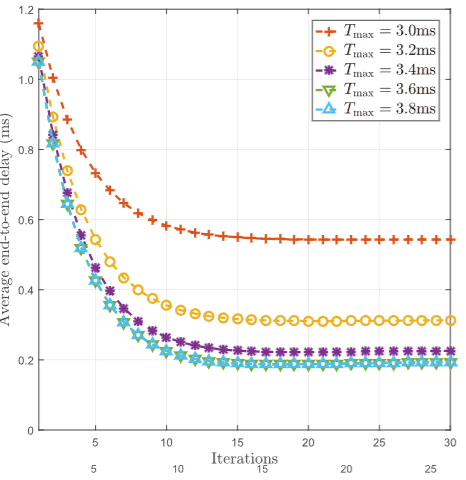
\includegraphics[width=0.75\linewidth]{image4.png}
    \caption{}
    \label{fig:placeholder4}
\end{figure}
\end{frame}

\begin{frame}{}
\small

\begin{itemize}
    \item The paper plots average end-to-end delay versus FaBo iterations.
    \item FaBo converges to the minimum delay in about:
    \[
    15 \text{ iterations}
    \]

    \item This means the flexible proximal ADMM update reaches a stable blocklength solution quickly.

    \item The result supports the claim that FaBo is suitable for low-latency systems.

    \item The paper also observes that as $T_{\max}$ increases:
    \[
    D_{\text{aver}}^{su}
    \text{ first decreases and then becomes stable.}
    \]

    \item Interpretation:
    \[
    \text{too small } T_{\max} \Rightarrow \text{not enough service time}
    \]
    \[
    \text{sufficient } T_{\max} \Rightarrow \text{delay cannot improve much further}
    \]
\end{itemize}

\end{frame}

\begin{frame}{FaBo Result 2: Choosing the Number of Frames}
\begin{figure}
    \centering
    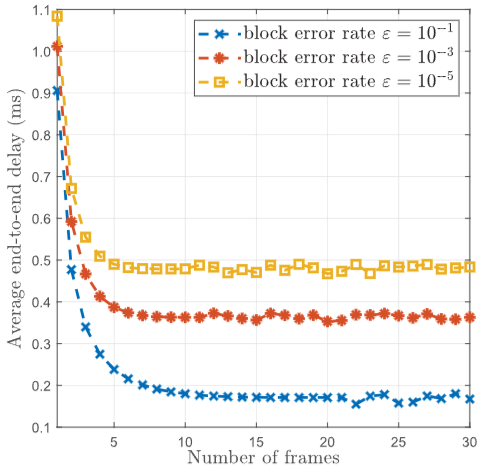
\includegraphics[width=0.75\linewidth]{image5.png}
    \label{fig:placeholder5}
\end{figure}
\end{frame}

\begin{frame}{}
\small

\begin{itemize}
    \item The paper studies delay versus the number of frames $L$.
    \item As $L$ increases:
    \[
    D_{\text{aver}}^{su}
    \text{ first decreases, then converges.}
    \]

    \item Reason:
    \[
    L \uparrow
    \Rightarrow
    \text{more flexibility in choosing adaptive frame lengths}
    \]

    \item But after a point, extra frames receive zero or negligible blocklength.

    \item The optimal effective number of frames is:
    \[
    L^* = \text{index of the last non-zero blocklength frame}
    \]

    \item Practical method:
    \[
    \text{choose a large } L,\ \text{run FaBo, then find last } n_i>0.
    \]
\end{itemize}

\end{frame}

\begin{frame}{FaBo Result 3: Blocklength Pattern}
\begin{figure}
    \centering
    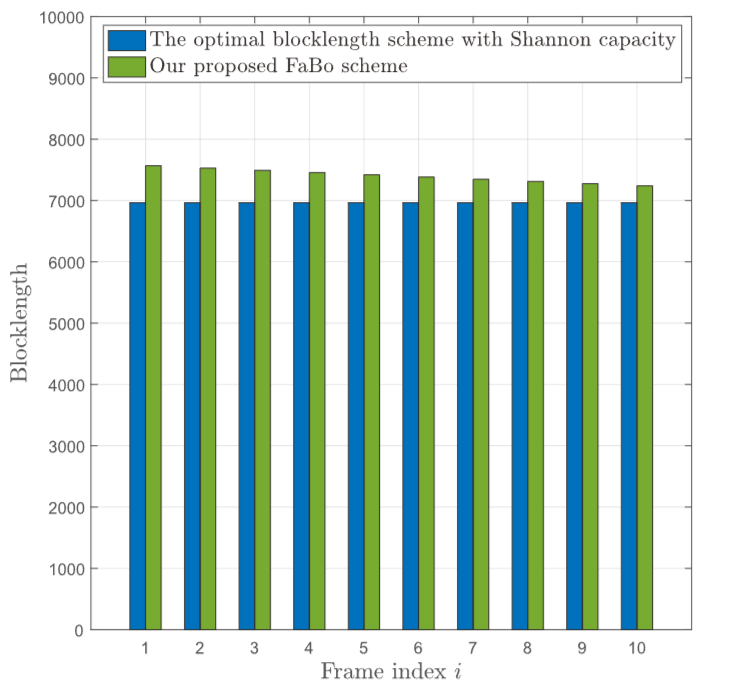
\includegraphics[width=0.75\linewidth]{image6.png}
    \label{fig:placeholder6}
\end{figure}
\end{frame}

\begin{frame}{}
\small

\begin{itemize}
    \item Earlier frames are longer:
    \[
    \text{large } n_i \Rightarrow \text{lower queing delay}
    \]

    \item This reduces queuing delay for early packets.

    \item Later frames are shorter:
    \[
    \text{small } n_i \Rightarrow \text{lower transmission delay}
    \]

    \item Therefore, FaBo balances:
    \[
    D_{\text{queue}}
    \quad \text{and} \quad
    D_{\text{trans}}
    \]
\end{itemize}

\end{frame}

\begin{frame}{FaBo Result 4: Comparison with 5G NR}

\begin{figure}
    \centering
    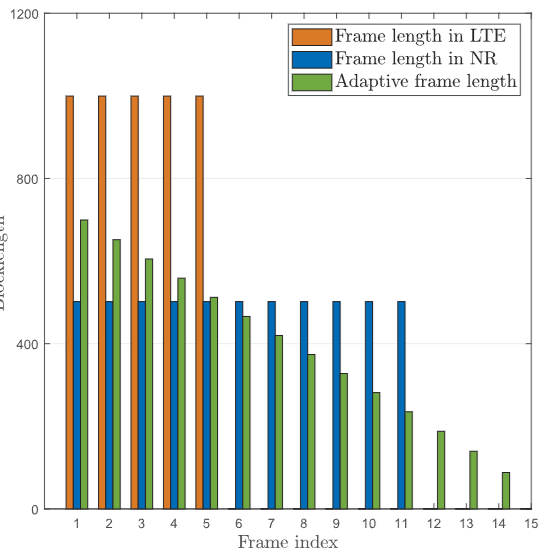
\includegraphics[width=0.75\linewidth]{image7.png}
    \caption{}
    \label{fig:placeholder7}
\end{figure}

\end{frame}

\begin{frame}{}
\small
\begin{itemize}
    \item The paper compares FaBo with fixed-blocklength 5G NR.
    \item 5G NR uses fixed TTI:
    \[
    T_{\text{NR}}=0.5\text{ ms}
    \]

    \item FaBo can have larger queuing delay than 5G NR:
    \[
    D_{\text{queue}}^{\text{FaBo}}
    >
    D_{\text{queue}}^{\text{NR}}
    \]

    \item But FaBo has much smaller transmission delay:
    \[
    D_{\text{trans}}^{\text{FaBo}}
    <
    D_{\text{trans}}^{\text{NR}}
    \]

    \item Overall:
    \[
    D_{\text{E2E}}^{\text{FaBo}}
    <
    D_{\text{E2E}}^{\text{NR}}
    \]

    \item This proves that minimizing only one delay component is not enough.
\end{itemize}

\end{frame}

\begin{frame}{FaBo Result 5: Comparison with LTE/NR Schemes}
\begin{figure}
    \centering
    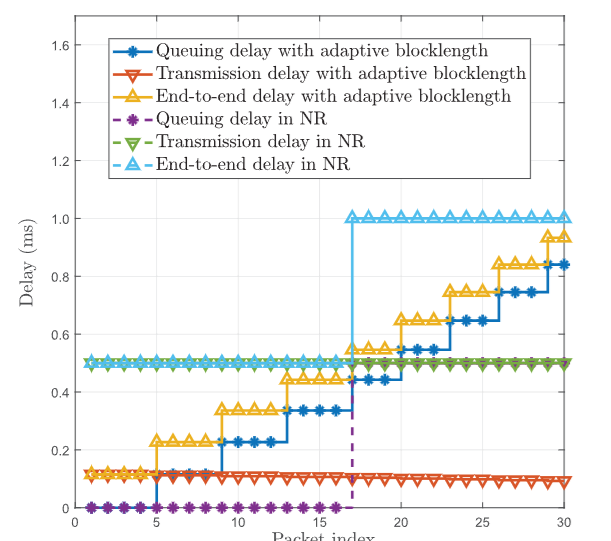
\includegraphics[width=0.75\linewidth]{image8.png}
    \label{fig:placeholder8}
\end{figure}
\end{frame}

\begin{frame}{}

\small

\begin{itemize}
    \item The paper compares FaBo against:
    \[
    \text{LTE long-frame scheme}
    \]
    \[
    \text{5G NR short-frame schemes}
    \]
    \[
    \text{one-packet-one-frame scheme}
    \]

    \item LTE long frame:
    \[
    T=1\text{ ms}
    \]

    \item 5G NR short frames:
    \[
    T=0.5,\ 0.25,\ 0.125,\ 0.0625\text{ ms}
    \]

    \item FaBo achieves smaller average end-to-end delay than fixed-frame schemes.

    \item fixed TTI cannot adapt to packet queue and rate tradeoff

    \item FaBo adapts each frame length according to the delay objective.
\end{itemize}

\end{frame}

\begin{frame}{FaBo Results: Main Inference}
\small

\begin{itemize}
    \item FaBo converges quickly:
    \[
    \approx 15 \text{ iterations}
    \]

    \item It identifies the effective number of useful frames:
    \[
    L^* = \text{last non-zero } n_i
    \]

    \item It produces decreasing frame lengths:
    \[
    n_1>n_2>\cdots
    \]

    \item Long early frames reduce queuing delay:
    \[
    R(n_i)n_i \uparrow
    \Rightarrow
    \text{more packets served early}
    \]

    \item Short later frames reduce transmission delay.

    \item Final conclusion: Adaptive blocklength gives better end to end latency by better queuing-transmission delay balance than fixed LTE/NR TTI.
\end{itemize}

\end{frame}

\section{Comparison with our method}

\begin{frame}{Comparison with our method: Paper 1}
\begin{itemize}
    \item This paper optimizes for the sum rate under latency constraints by finding the optimal precoder while we directly optimize for the latency.
    \item The blocklength is fixed and only the precoder is optimized.
    \item Paper uses lower bound for FBL Rate to find first order optimal solution this is problematic since the assumptions are too extreme (such as treating the SNR as constant when it depends on the precoder), however we keep the non-convex FBL rate and find the optimal solution by parameterizing with NN and using gradient descent.
    \item Only delay constrained users are modeled using FBL rate while delay tolerant users are modeled with Shannon Rate and are assumed to have infinite blocklength. We model all users with FBL rate to mimize latency.
\end{itemize}

\end{frame}

\begin{frame}{Comparison with our method: Paper 2}
\begin{itemize}
    \item Paper assumes bits per packet based continuous transmission while we assume large payload of bits that are split between sub-block coherant channels.
    \item This paper does directly optimize for the latency but only by optimizing the blocklength while we optimize both precoder and blocklength to make a lower blocklength possible.
    \item Paper considers tradeoff with queing delay while we dont.
    \item Paper assumes fixed bits per packet and optimizes blocklength only.
    However we opt to fit as many bits into a sub-block as possible after finding the optimal precoder and sub-blocklength.
    This is because we recognize that fitting max bits into initial sub-block is optimal compared to having a lower blocklength to reduce latency.
    This is due to the fact that even though maximizing bits and reducing symbols result in the same purpose of increasing bits/symbol and thus reducing latency they have different effects on the FBL rate inequality equation.
\end{itemize}

\end{frame}

\end{document}
